\documentclass[]{article}
\usepackage{polski}
\usepackage[utf8]{inputenc}
\usepackage{amsmath}
\usepackage{graphicx}
\usepackage{caption}
\usepackage{subcaption}
\usepackage{geometry}
\usepackage{float}

\geometry{legalpaper, margin=0.6in}


%opening
\title{TST - Projekt 1}
\author{Jakub Postępski}

\begin{document}

\maketitle


\section{Wprowadzenie}
Przyjmijmy macierz $A_{2x2}$.

Macierz posiada, dla $i = {1, 2}$:
\begin{itemize}
	\item wartości własne $\lambda_i$
	\item wektory własne $\vec{v_i}$
\end{itemize}

W zadaniu interesuje nas dynamika ciągu:
\[x^{(t)} = A^tx_0 \]

\section{Wartości własne}

Podstawowym równaniem jest:
\[ Ax = \lambda x\]

Zbiór rozwiązań opisany równaniem charakterystycznym:

\[ \varphi_A(z) = det(zI-A) \]

to widmo: 
\[\sigma(A) = \{ \lambda_i \in \  \textbf{C}\} \]

Szukamy wartości dla których macierz $A$ zachowa się jak przekształcenie liniowe (skalar). Dla takich wartości macierz tylko powiększa lub zmniejsza zadany wektor, ale nie zależności pomiędzy składowymi wektora.

Z równania wynika, że wartości własne decydują o tym jakim przekształceniem będzie macierz $A$.

\section{Wektory własne}
Są wektorami rozpinającymi bazę którą tworzy przekształcenie macierzy A. Zestaw takich wektorów nie jest jednoznaczny. Dla jednej macierzy można znaleźć wiele zestawów wektorów rozpinających. Wektory własne decydują więc o obrocie (konfiguracji) naszego przekształcenia.

\section{Związek wartości i wektorów własnych}
Wiemy już, że wartości własne (poniżej zapisane w diagonalnej macierzy $D$) definiują przekształcenie, a zestaw wektorów własnych (poniżej zapisane w macierzy $V$) jego obrót. Aby przekształcenie zachowywało się tak samo (pod względem widma) jak $D$ musi zachodzić (szukamy macierzy podobnej):
\[A = VDV^{-1}\]

dzięki czemu jesteśmy w stanie znaleźć macierz $A$.


\section{Dynamika układów}
\subsection{Przykładowy układ}
\begin{figure}[H]
	\centering
	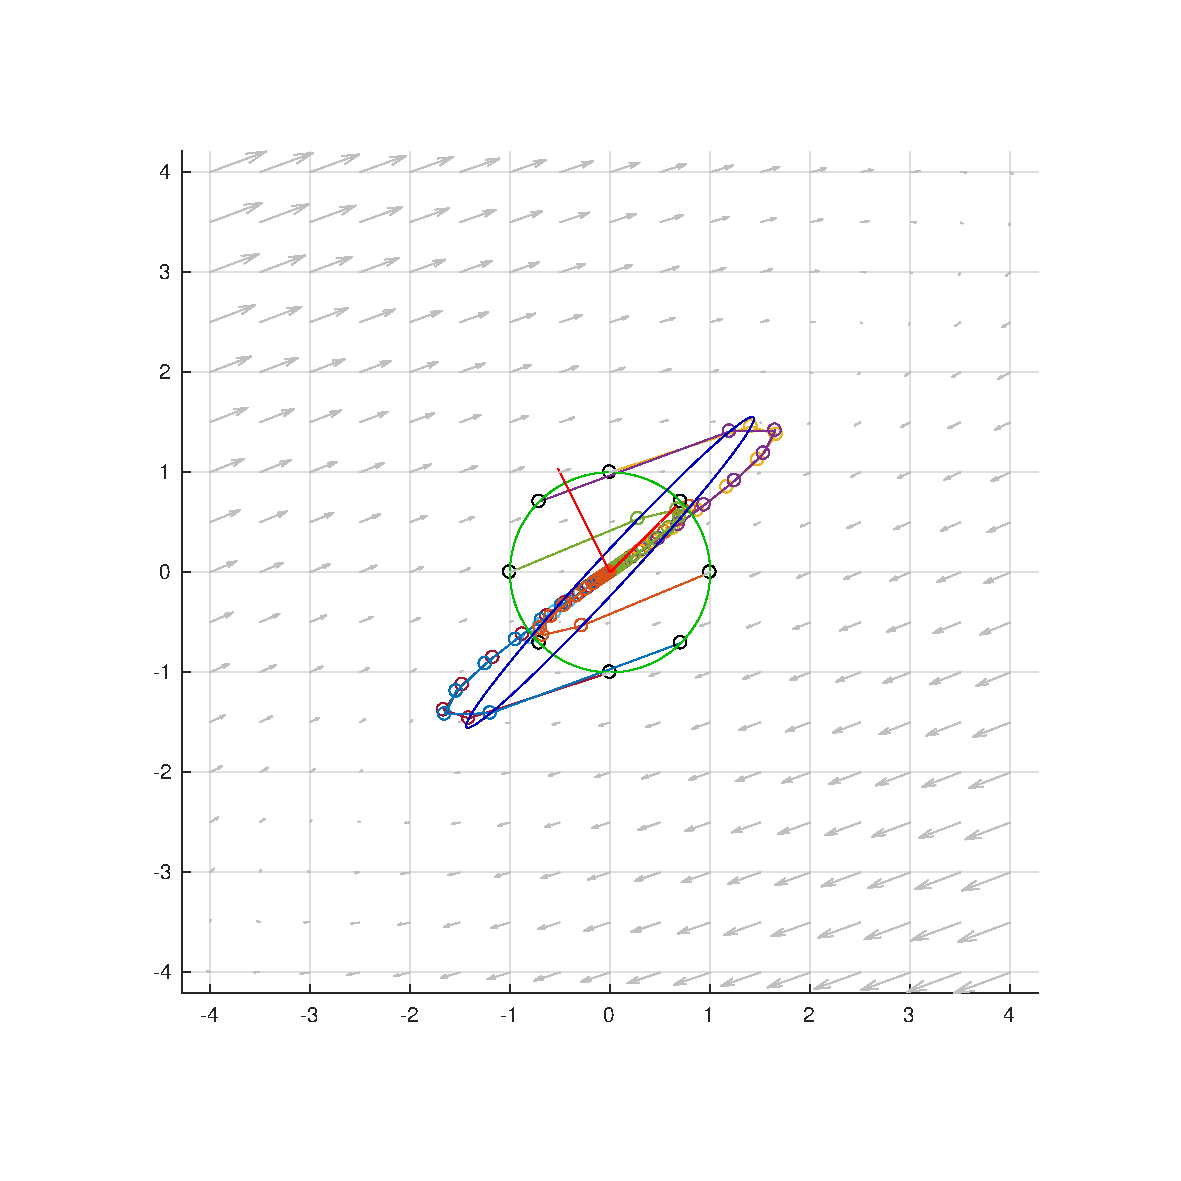
\includegraphics[width=0.99\linewidth]{demo}
	\caption{Przykładowy układ z losowymi wartościami. "Popychany" przez gradient układ zbiega do zera, zgodnie z wyznaczonym obrazem.}
	\label{fig:normal0}
\end{figure}

\begin{figure}[H]
	\centering
	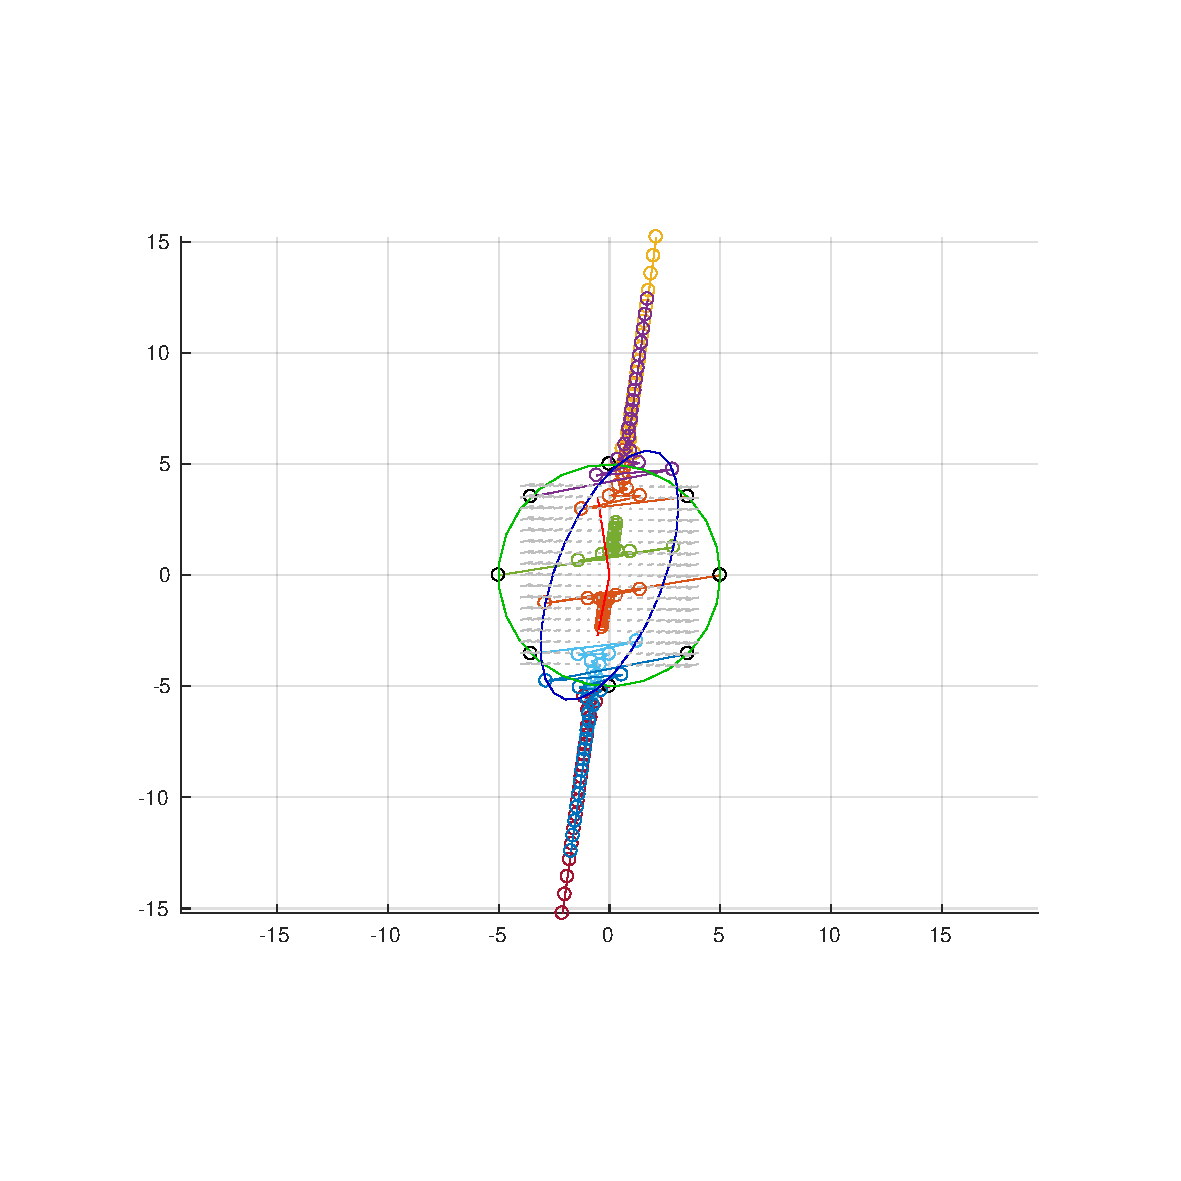
\includegraphics[width=0.99\linewidth]{demo3}
	\caption{Układ z losowymi wartościami. Jedne punkt startowy, $\lambda_1=1.0591 \lambda_2=-0.5435 $}
	\label{fig:demo2}
\end{figure}

\begin{figure}[H]
	\centering
	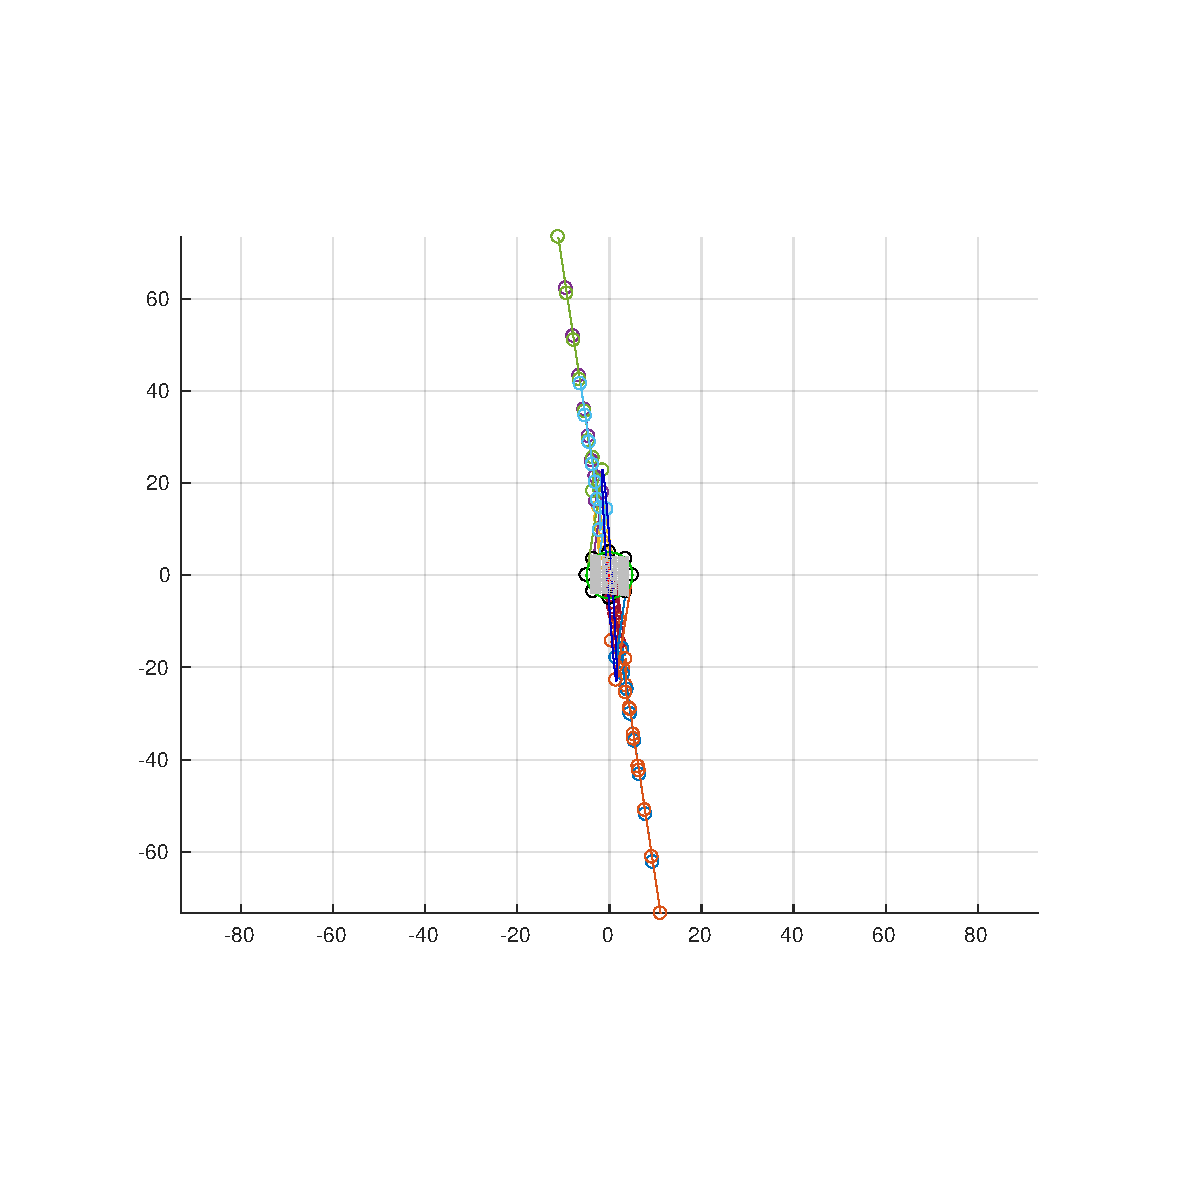
\includegraphics[width=0.99\linewidth]{linear}
	\caption{Układ przekształcenia liniowego, $\lambda_1=1.2 \lambda_2=-0.4 $}
	\label{fig:linear}
\end{figure}

\subsection{Postać widma}
Gdy macierz A jest postaci:
\[ A = \begin{bmatrix} a_{11} & a_{12} \\ a_{21} & a_{22} \end{bmatrix} \]
to równanie charakterystyczne:
\[ \varphi_A(\lambda) = (1-a_{11})(a_{22}) -a_{12}a_{21} \]
może mieć następujące wartości własne
\begin{itemize}
	\item dwie różne wartości rzeczywiste
	\item dwie jednakowe wartości rzeczywiste
	\item dwie sprzężone liczby zespolone
\end{itemize}
\begin{figure}[H]
	
	\centering
	\begin{subfigure}{.5\textwidth}
		\centering
		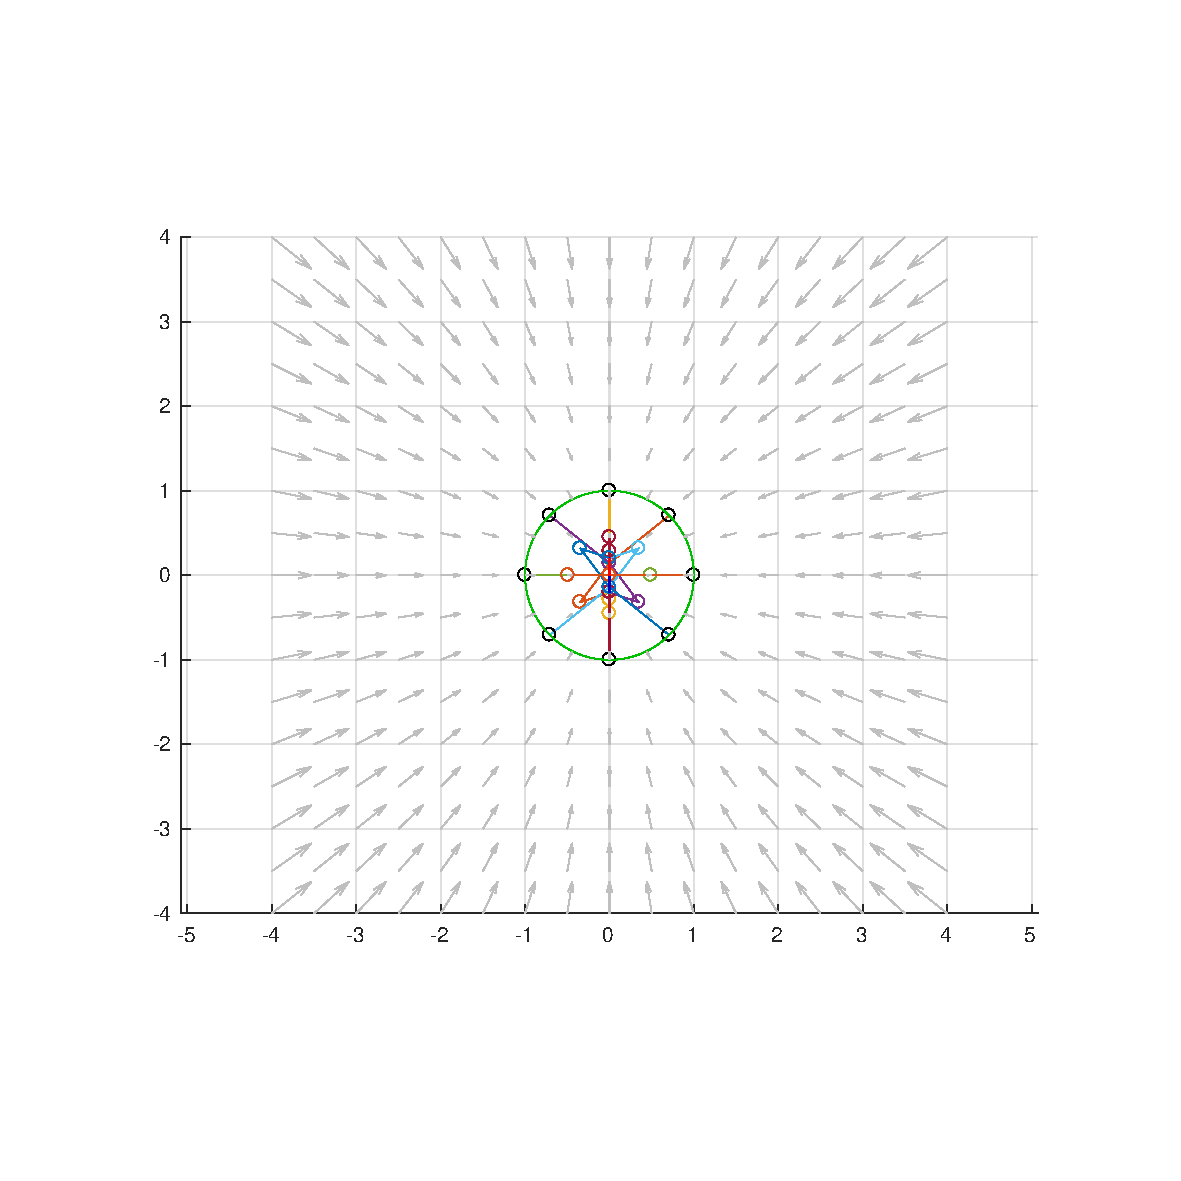
\includegraphics[width=0.99\linewidth]{imag_ok}
		\caption{Wartości zadne przez nas: $\lambda_1 = -0.7i, \lambda_2 = 0.2 + 0.7i $, Próba uzyskania wartości własnych funkcją eig() kończy się śmiercią programu matlaba (naprawdę!) albo ostrzeżeniem.}
		\label{fig:imag2}
	\end{subfigure}
	\begin{subfigure}{.5\textwidth}
		\centering
		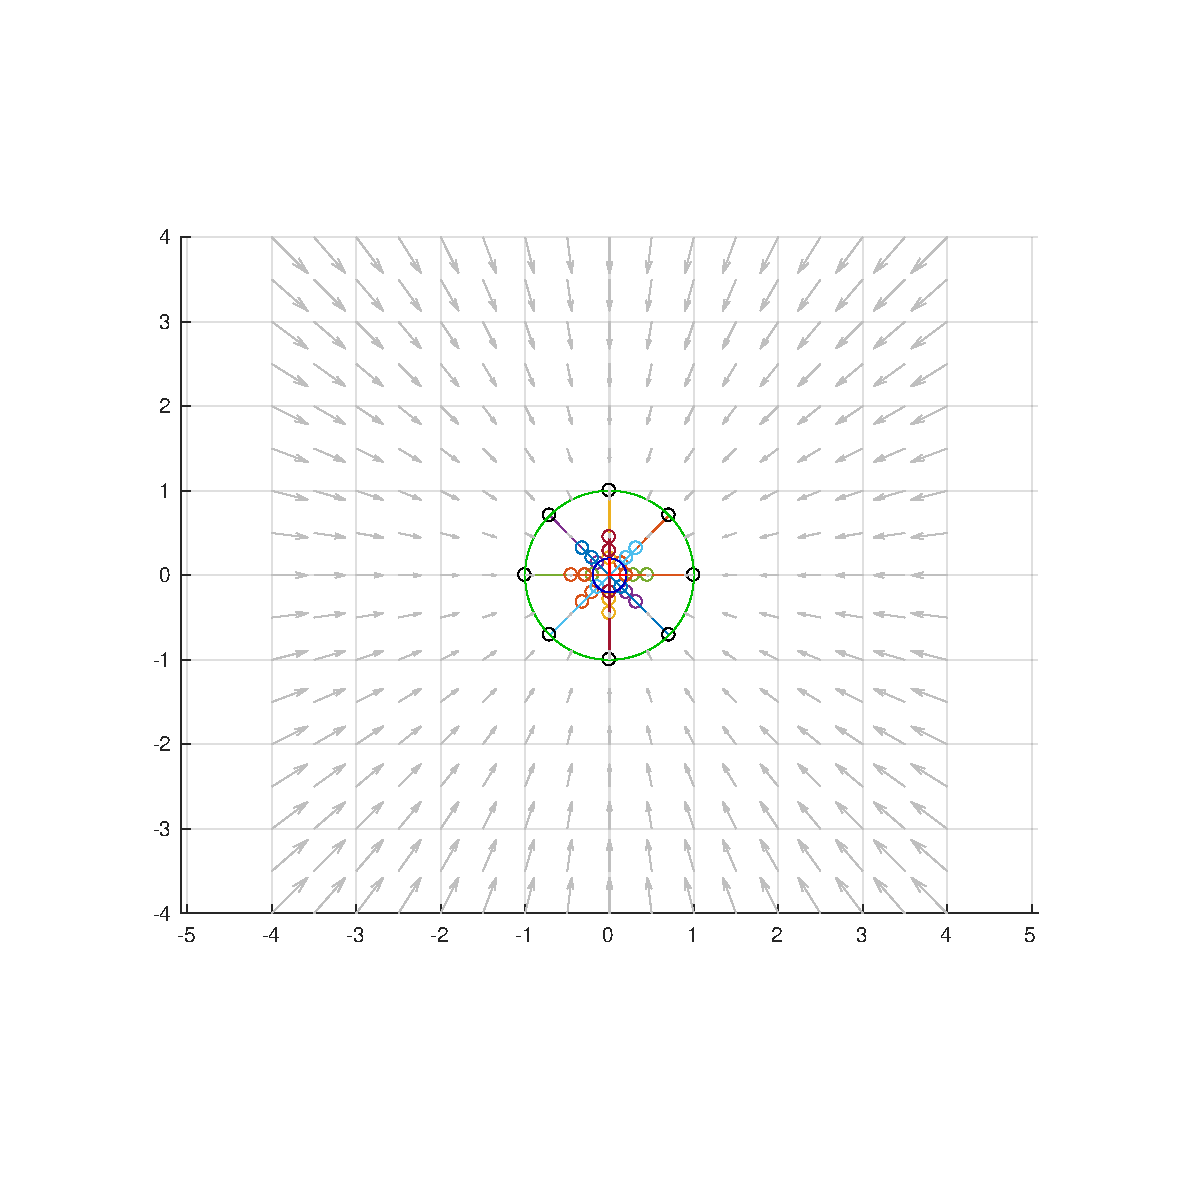
\includegraphics[width=0.99\linewidth]{imag_wrong}
		\caption{$\lambda_1 = -0.7i, \lambda_2 = 0.2 + 0.7i $}
		\label{fig:imag_1}
	\end{subfigure}%
	\begin{subfigure}{.5\textwidth}
		\centering
		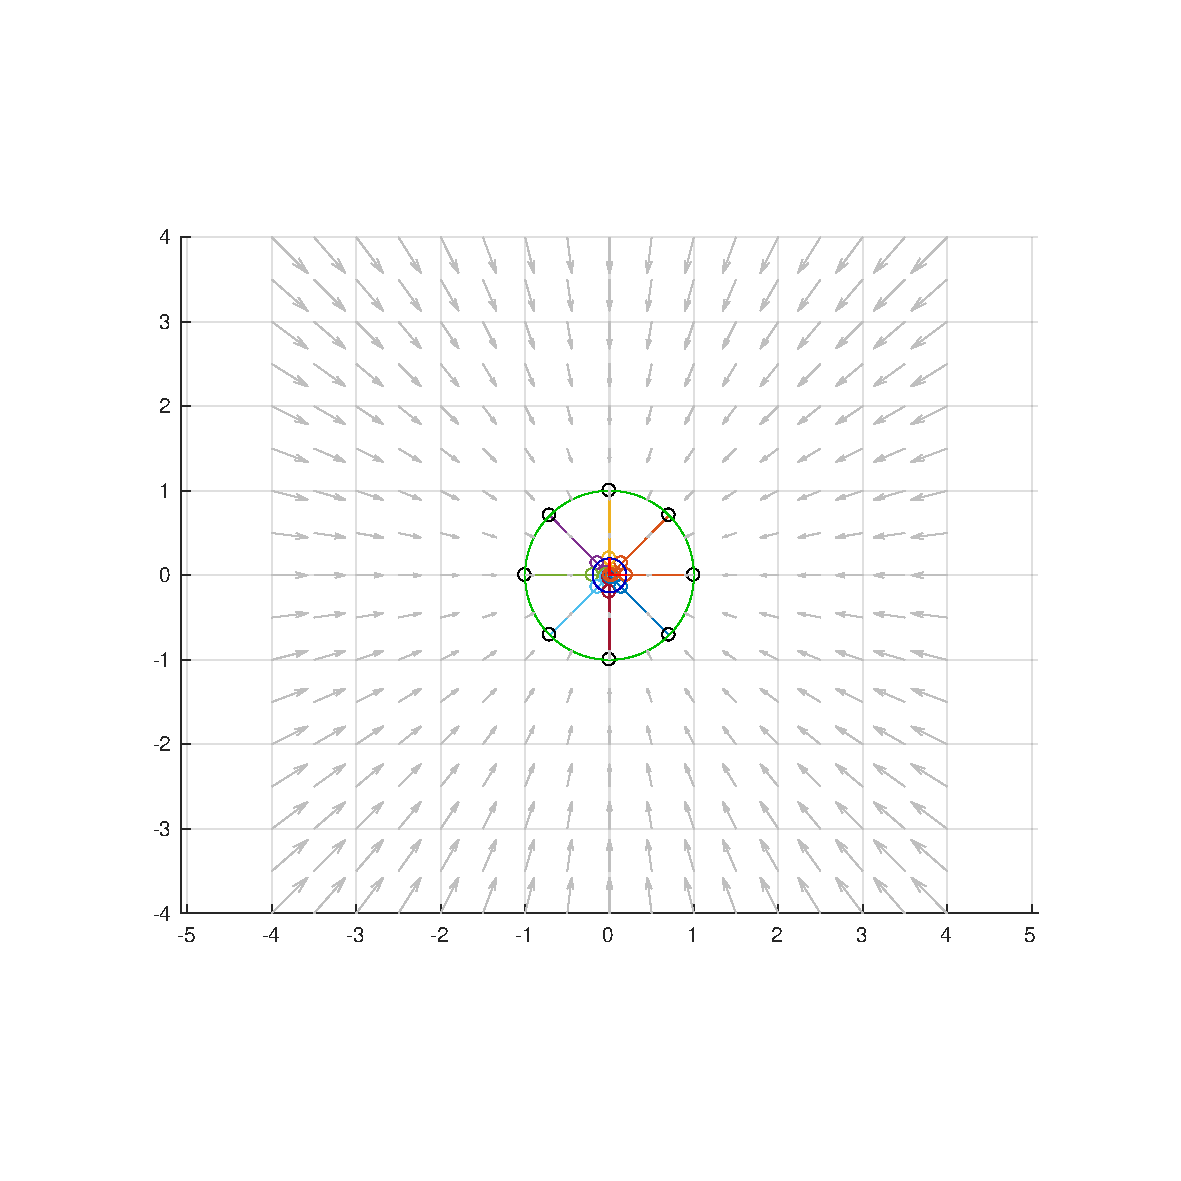
\includegraphics[width=0.99\linewidth]{imag_real}
		\caption{$\lambda_1 = 0.2, \lambda_2 = 0.2 $}
		\label{fig:imag_3}
	\end{subfigure}%
	\caption{Bieguny zespolone.}
	\label{fig3}
\end{figure}

\begin{figure}[H]
	\centering
	\begin{subfigure}{.5\textwidth}
		\centering
		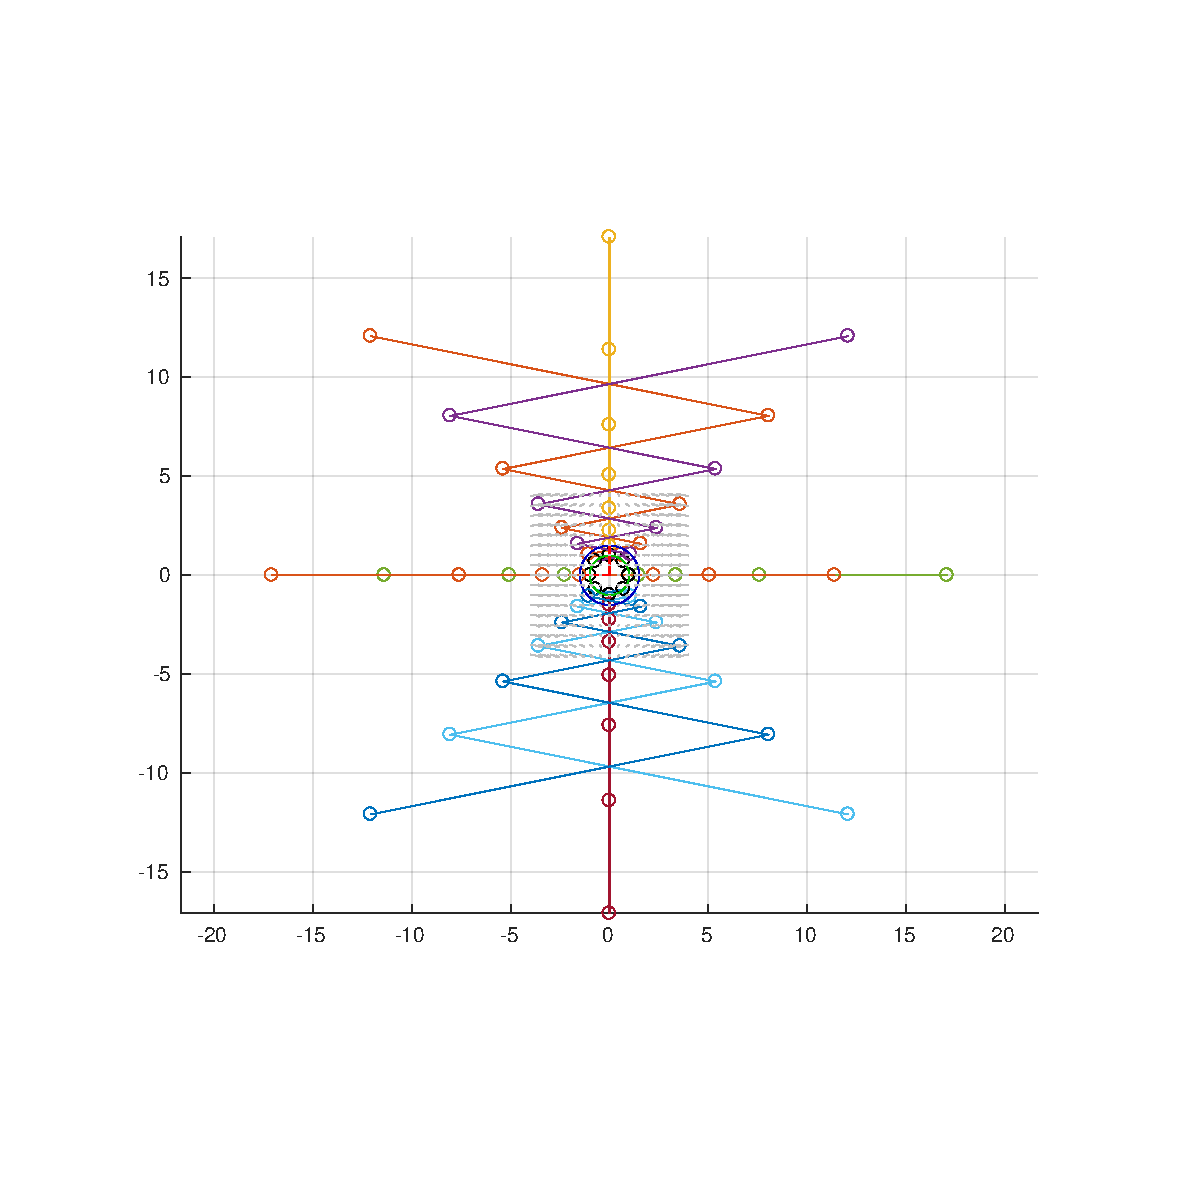
\includegraphics[width=0.99\linewidth]{imag_osc2}
		\caption{$\lambda_1 = -1.5, \lambda_2 = 1.5$}
		\label{fig:imag_osc}
	\end{subfigure}%
	\begin{subfigure}{.5\textwidth}
		\centering
		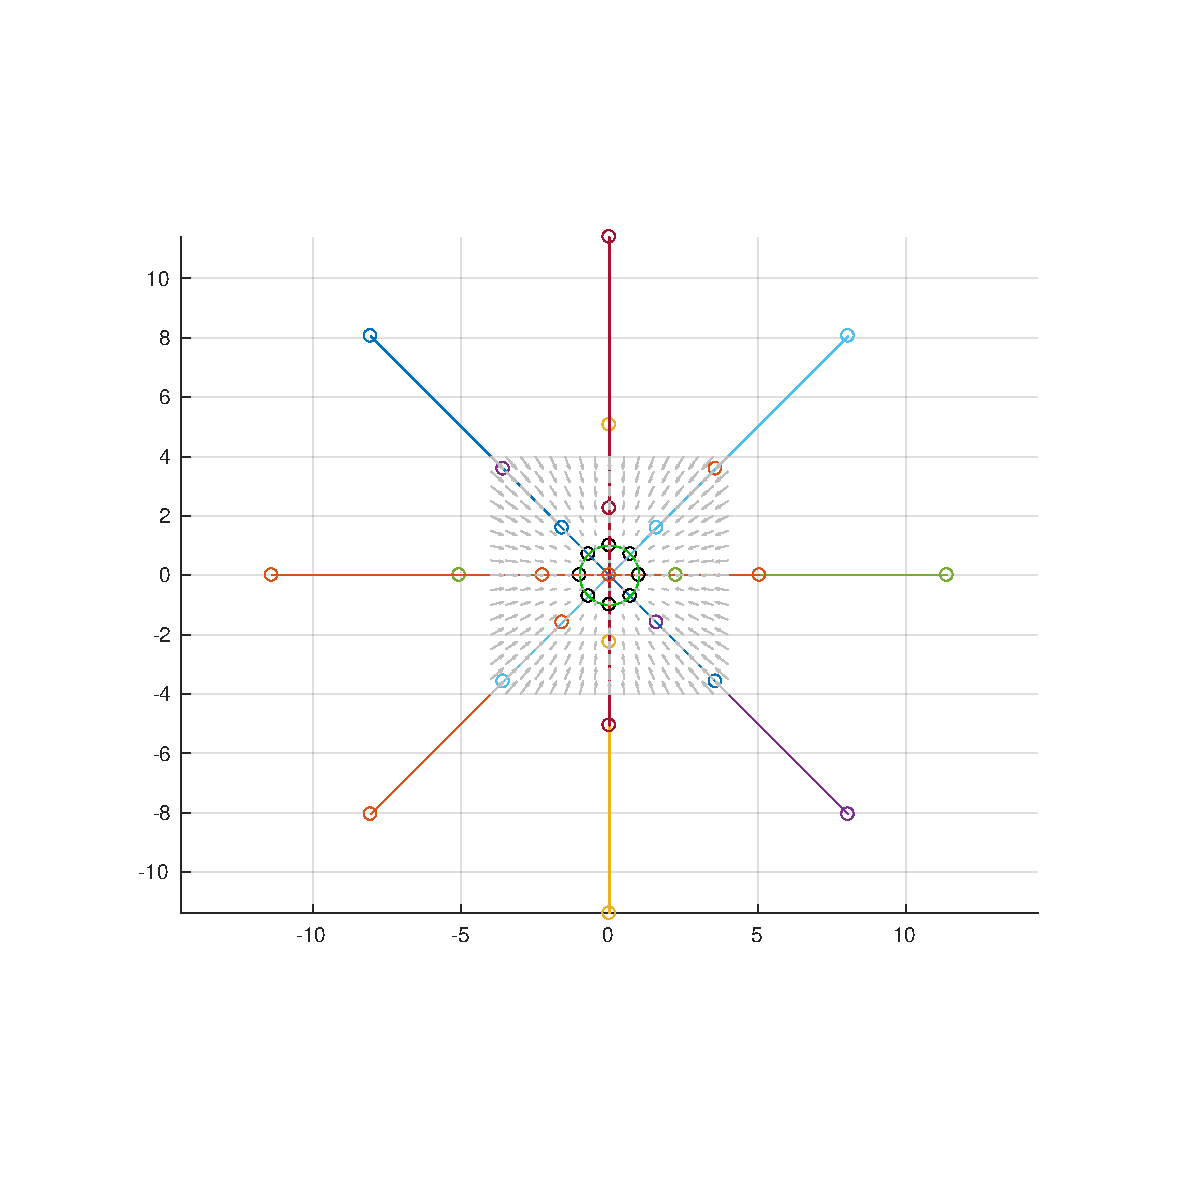
\includegraphics[width=0.99\linewidth]{imag_rot}
		\caption{$\lambda_1 = -1.5i, \lambda_2 = 1.5i$}
		\label{fig:imag_rot}
	\end{subfigure}
	\caption{Por: Układ wprowadzany jest w oscylacje nieuporządkowane; Trajektorie układu zamieniają się miejscami.}
	\label{fig5}
\end{figure}

W przypadku zastosowania liczb zespolonych można wpłynąć na obrót punktów trajektorii.

\subsection{Zastosowanie róznych wektorów własnych}

\begin{figure}[H]
	\centering
 	\begin{subfigure}{.5\textwidth}
		\centering
		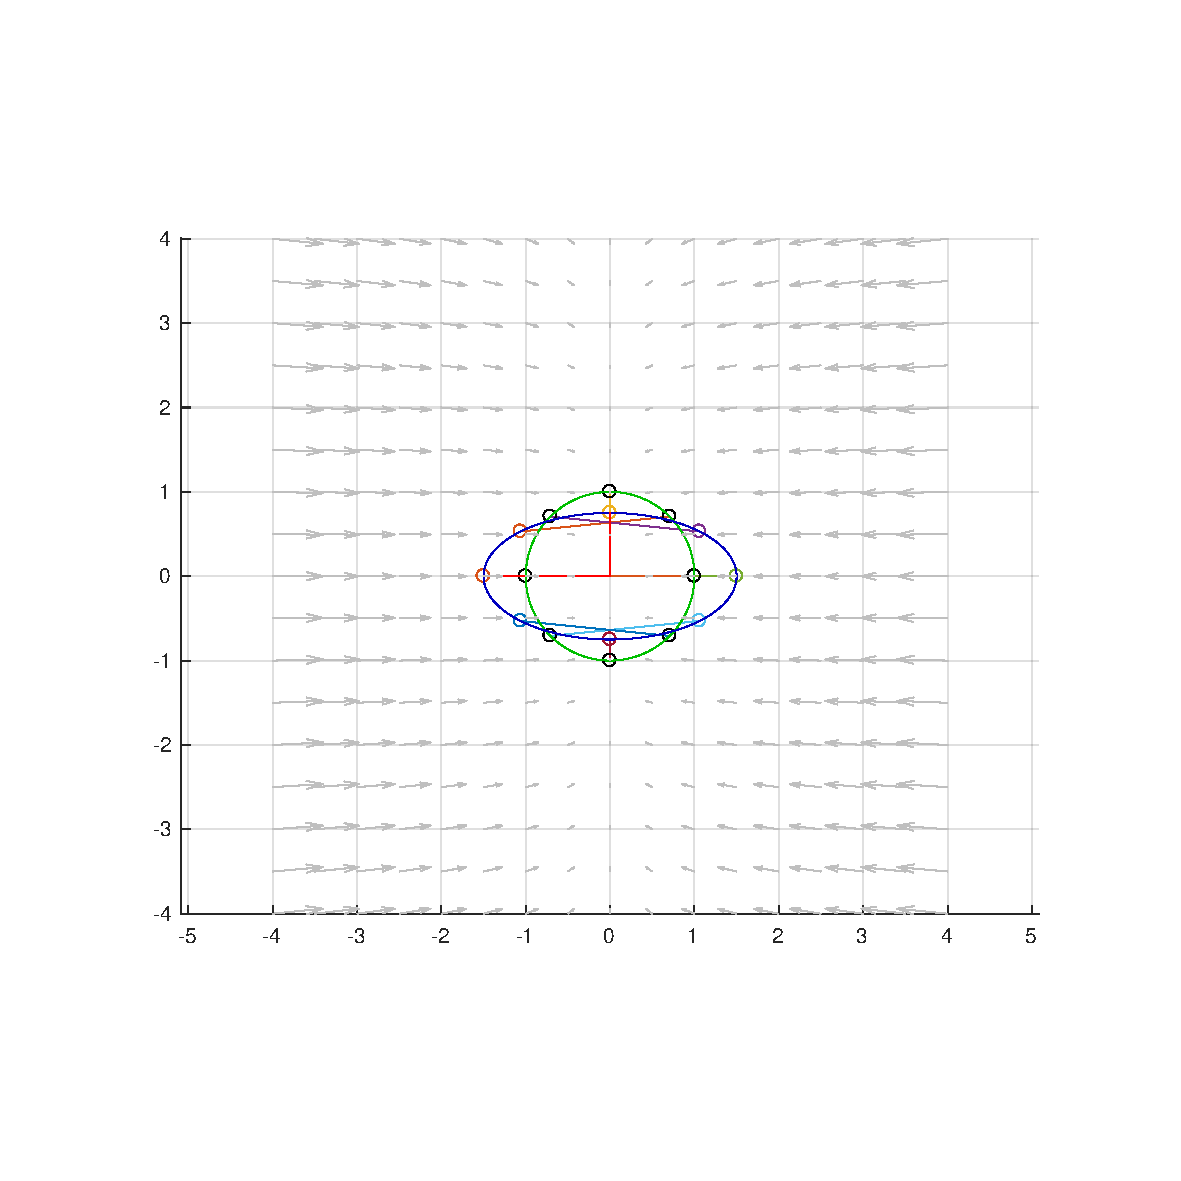
\includegraphics[width=0.99\linewidth]{normal_075_-15}
		\caption{$\lambda_1 = 0.75, \lambda_2 = -1.5$}
		\label{fig:rotation1}
	\end{subfigure}%
	\begin{subfigure}{.5\textwidth}
		\centering
		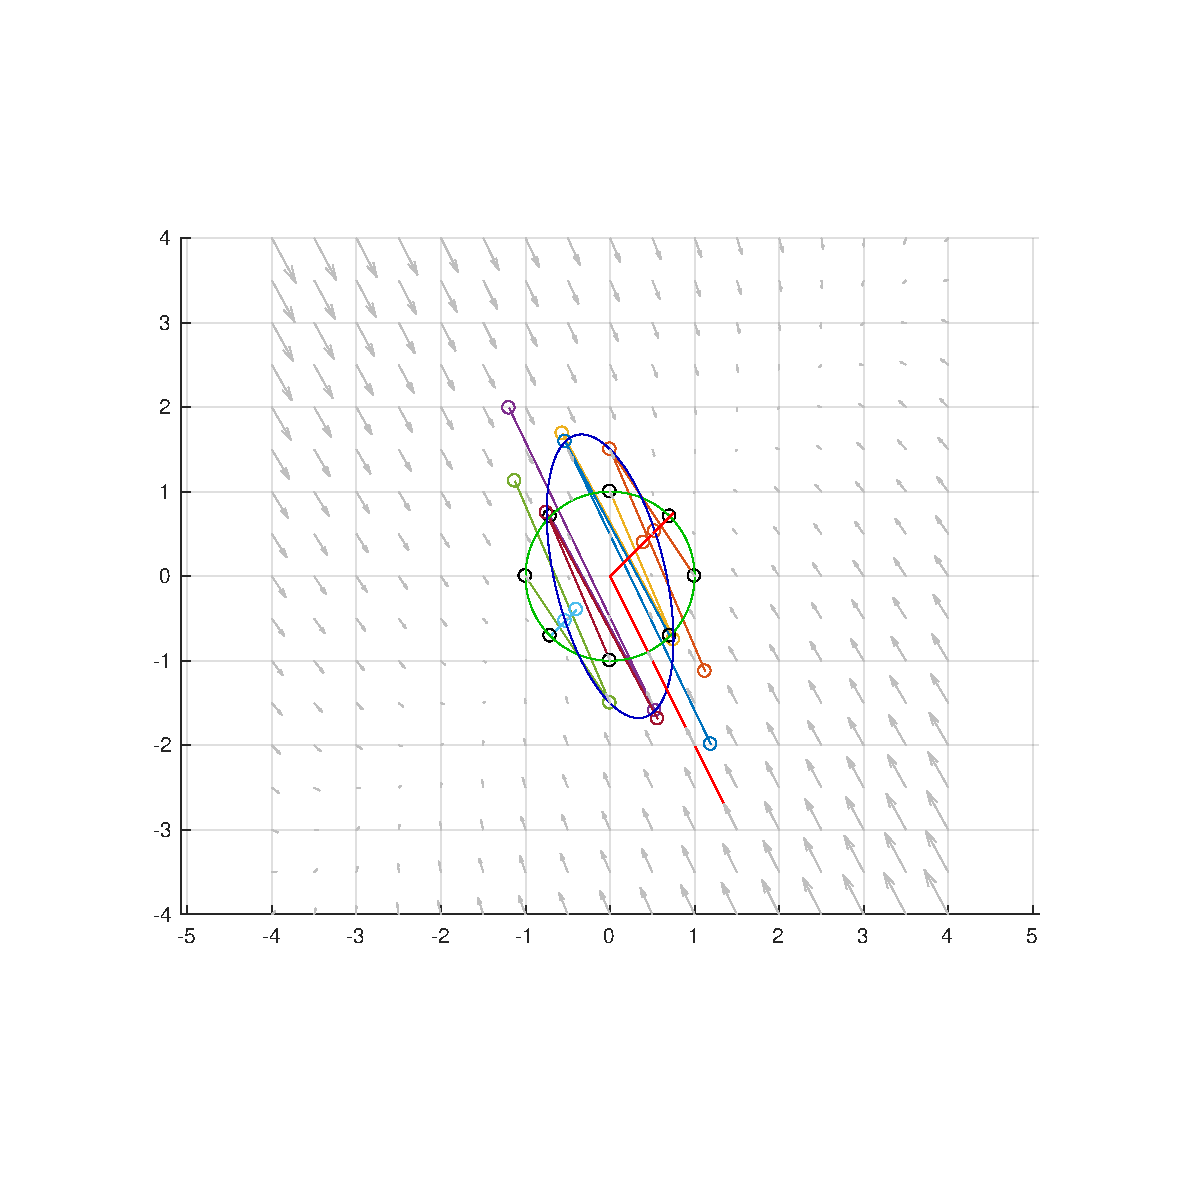
\includegraphics[width=0.99\linewidth]{rotated_075_-15}
		\caption{$\lambda_1 = 0.75, \lambda_2 = -1.5$}
		\label{fig:rotation2}
	\end{subfigure}
	\caption{Porównanie układów z jednakowymi wartościami własnymi. Różne wektory własne powodują obrót i przeskalowanie przekształcenia.}
	\label{fig1}
\end{figure}

\subsection{Stabilność układu}
Układ może być:
\begin{itemize}
	\item stabilny
	\item stabilny asymptotycznie\
	\item niestabilny
\end{itemize}

\begin{figure}[H]
	\centering
	\begin{subfigure}{.5\textwidth}
		\centering
		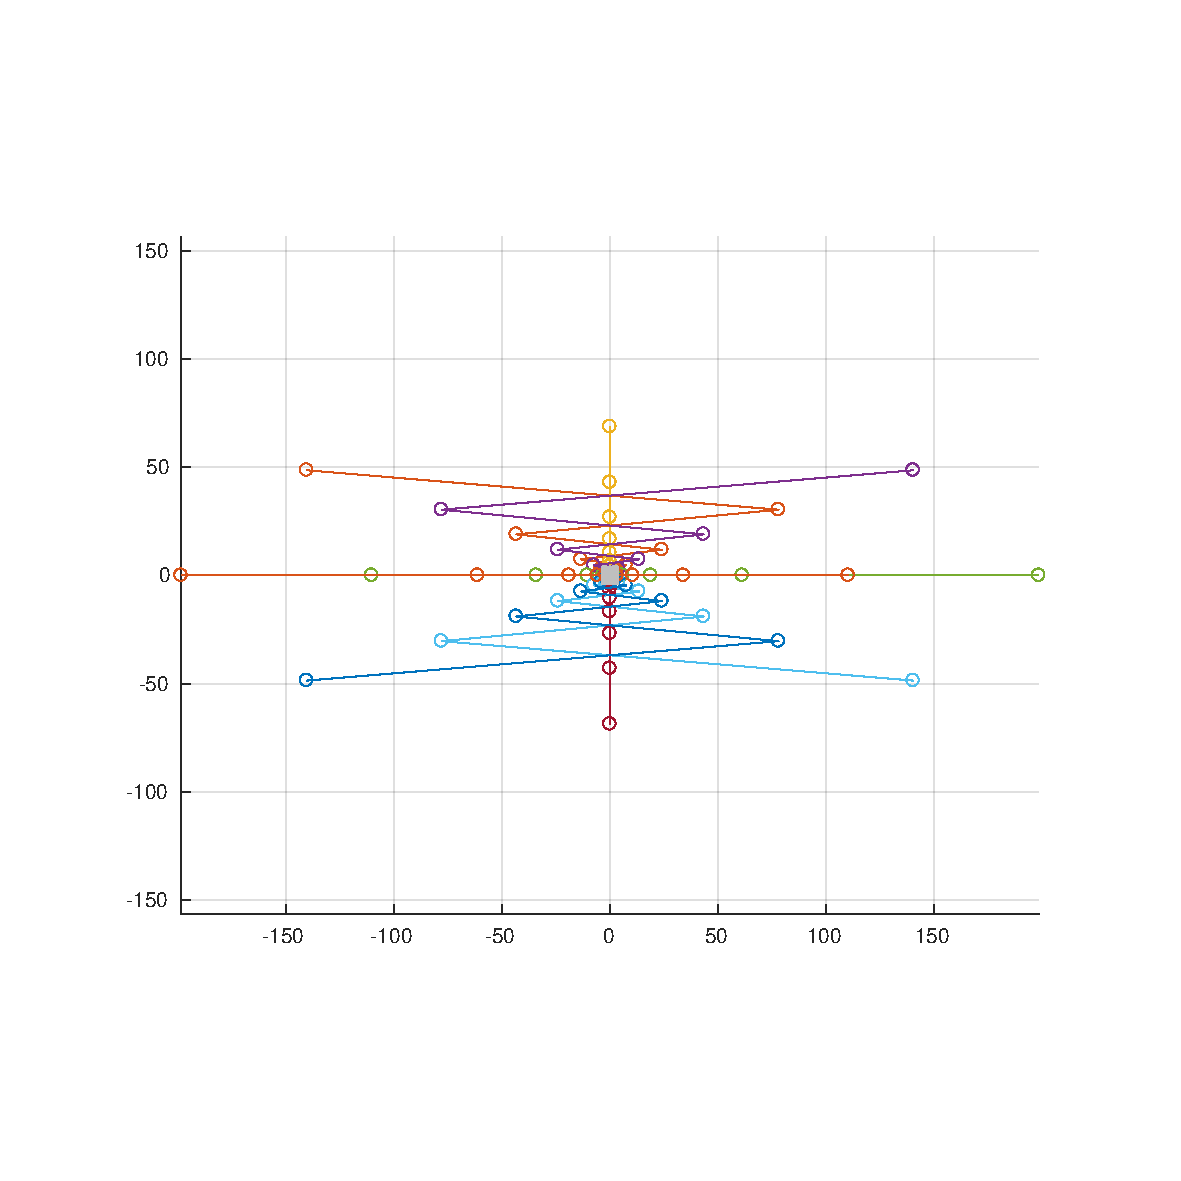
\includegraphics[width=0.99\linewidth]{normal_16_-18}
		\caption{$\lambda_1 = 1.6, \lambda_2 = -1.8$}
		\label{fig:normal1}
	\end{subfigure}%
	\begin{subfigure}{.5\textwidth}
		\centering
		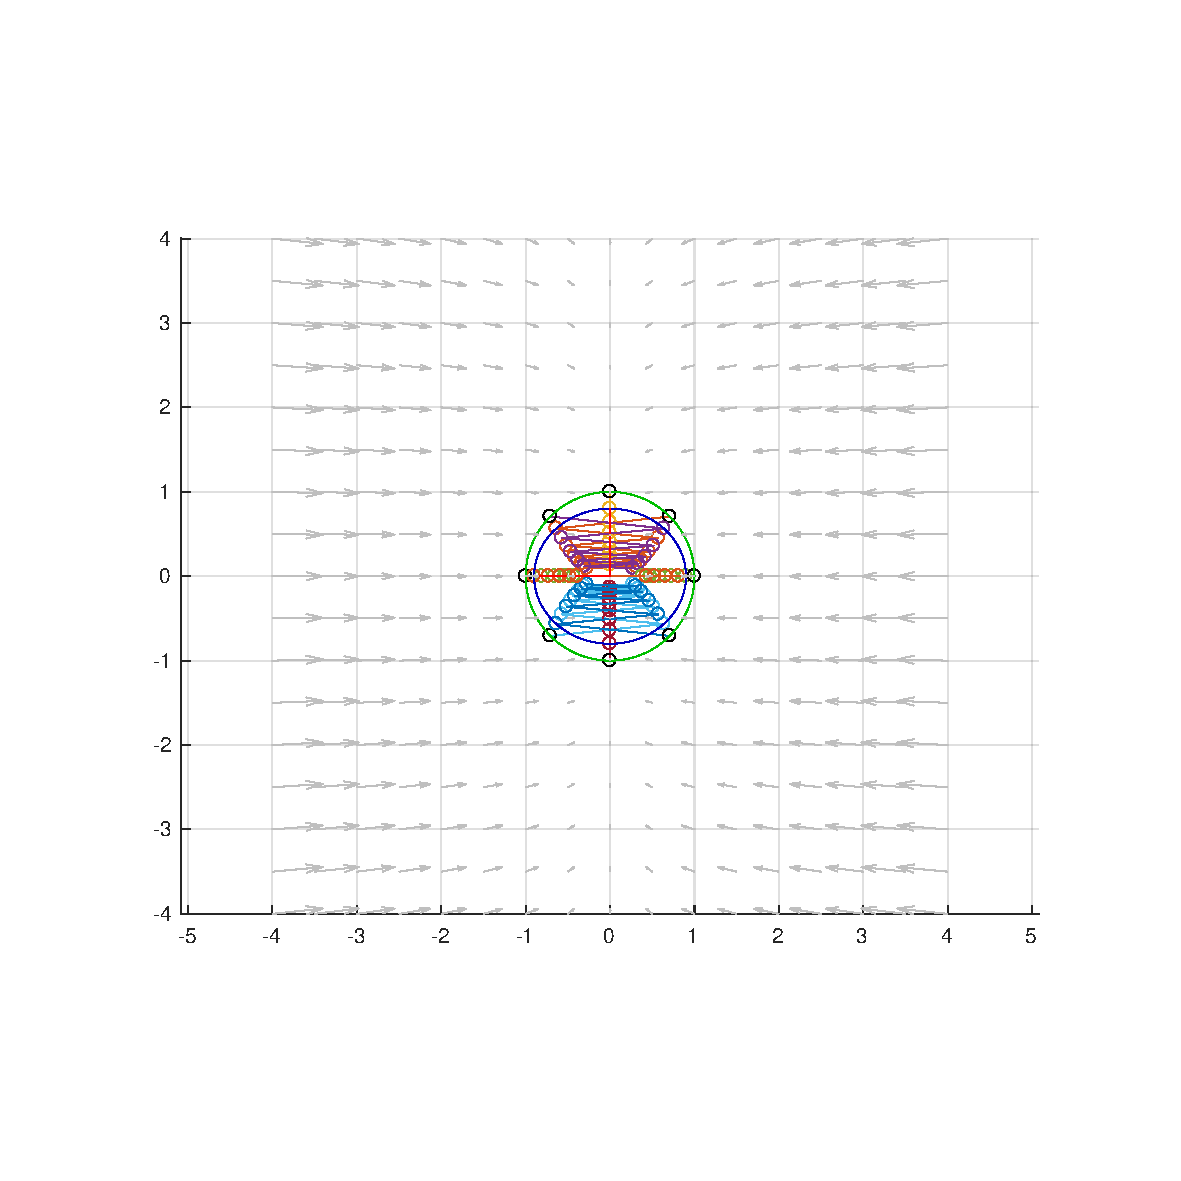
\includegraphics[width=0.99\linewidth]{normal_08_-09}
		\caption{$\lambda_1 = 0.8, \lambda_2 = -0.9$}
		\label{fig:normal2}
	\end{subfigure}
	\caption{Porównanie stabilności przy pomocy wartości spektralnych. W drugim przypadku $\rho < 1$. Por.: Układ rozbiega się; Układ zbiega do zera.}
	\label{fig2}
\end{figure}


\begin{figure}[H]
	\centering
	\begin{subfigure}{.5\textwidth}
		\centering
		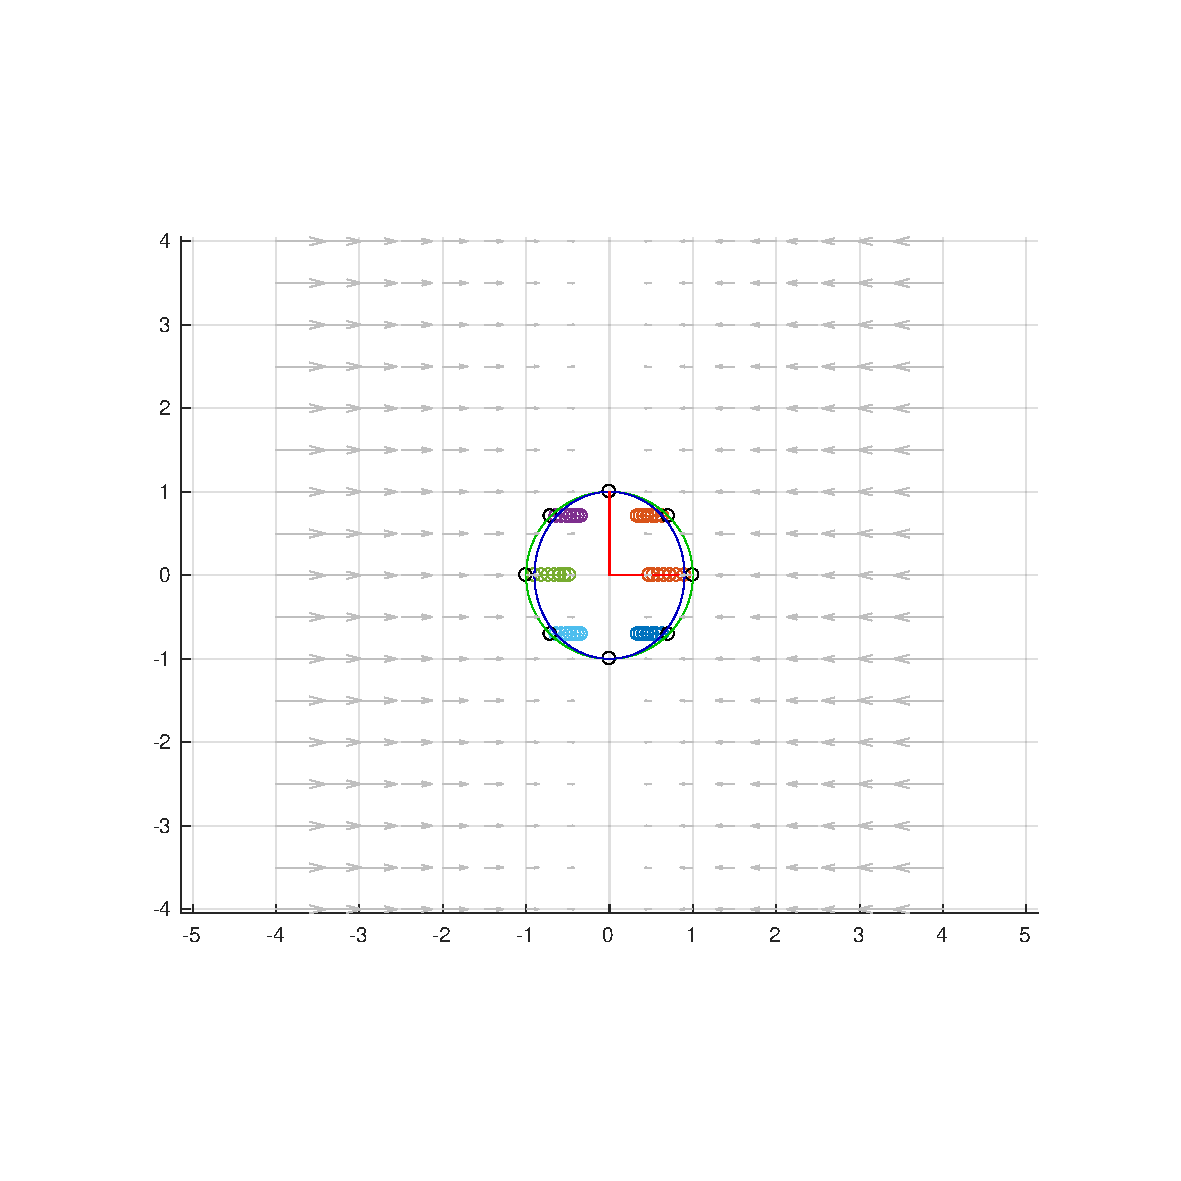
\includegraphics[width=0.99\linewidth]{const_9}
		\caption{$\lambda_1 = 0.9, \lambda_2 = 1 $}
		\label{fig:const1}
	\end{subfigure}
	\begin{subfigure}{.5\textwidth}
		\centering
		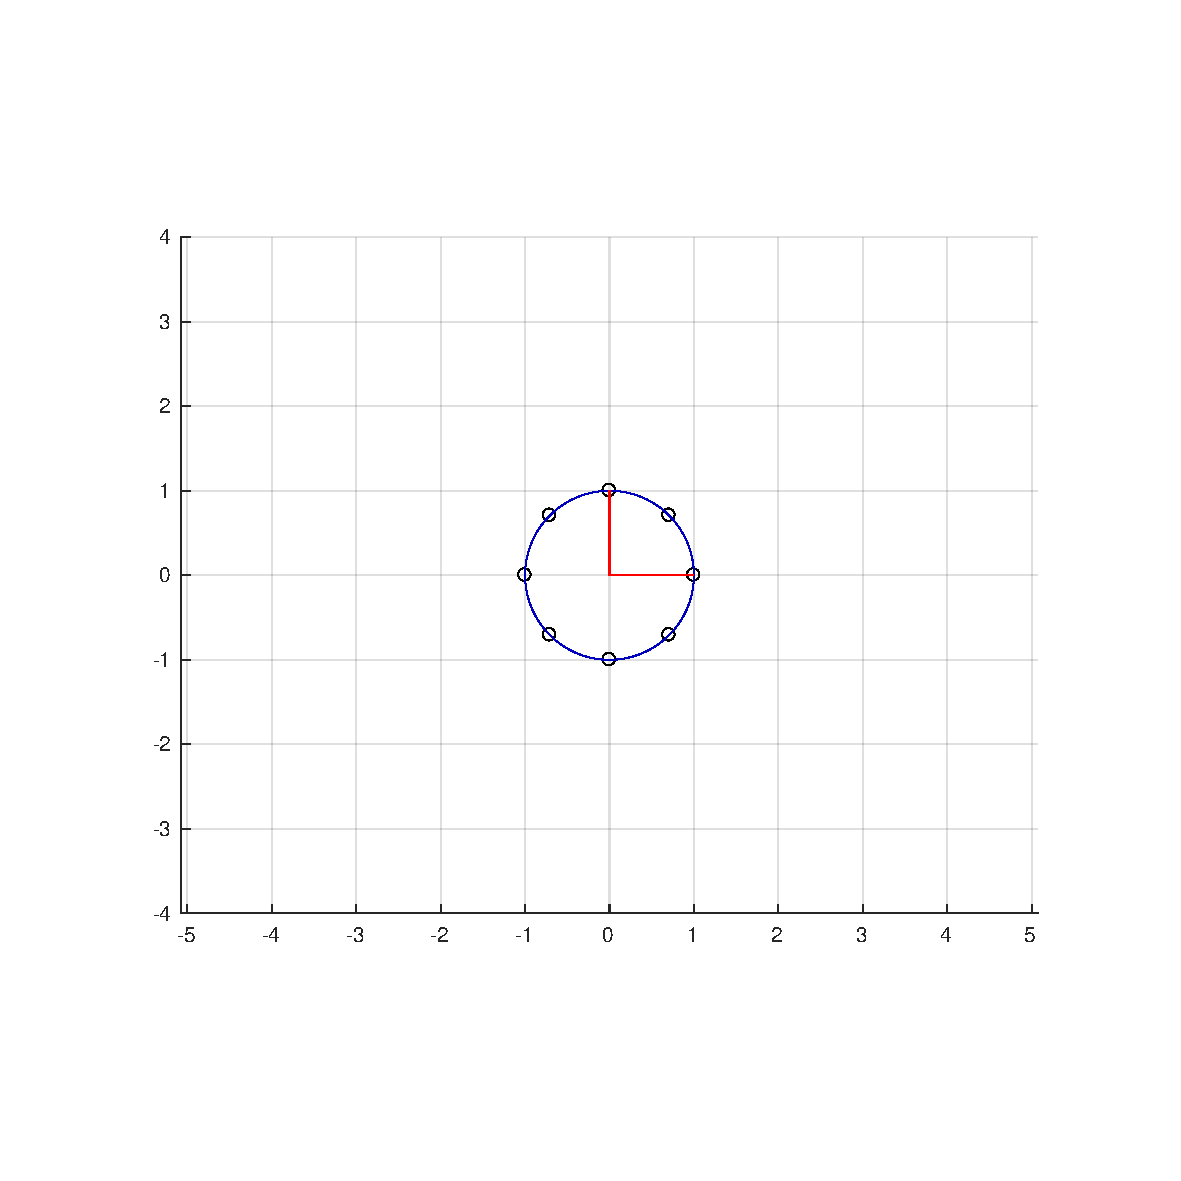
\includegraphics[width=0.99\linewidth]{const_10}
		\caption{$\lambda_1 = 1, \lambda_2 = 1 $}
		\label{fig:const2}
	\end{subfigure}%
	\begin{subfigure}{.5\textwidth}
		\centering
		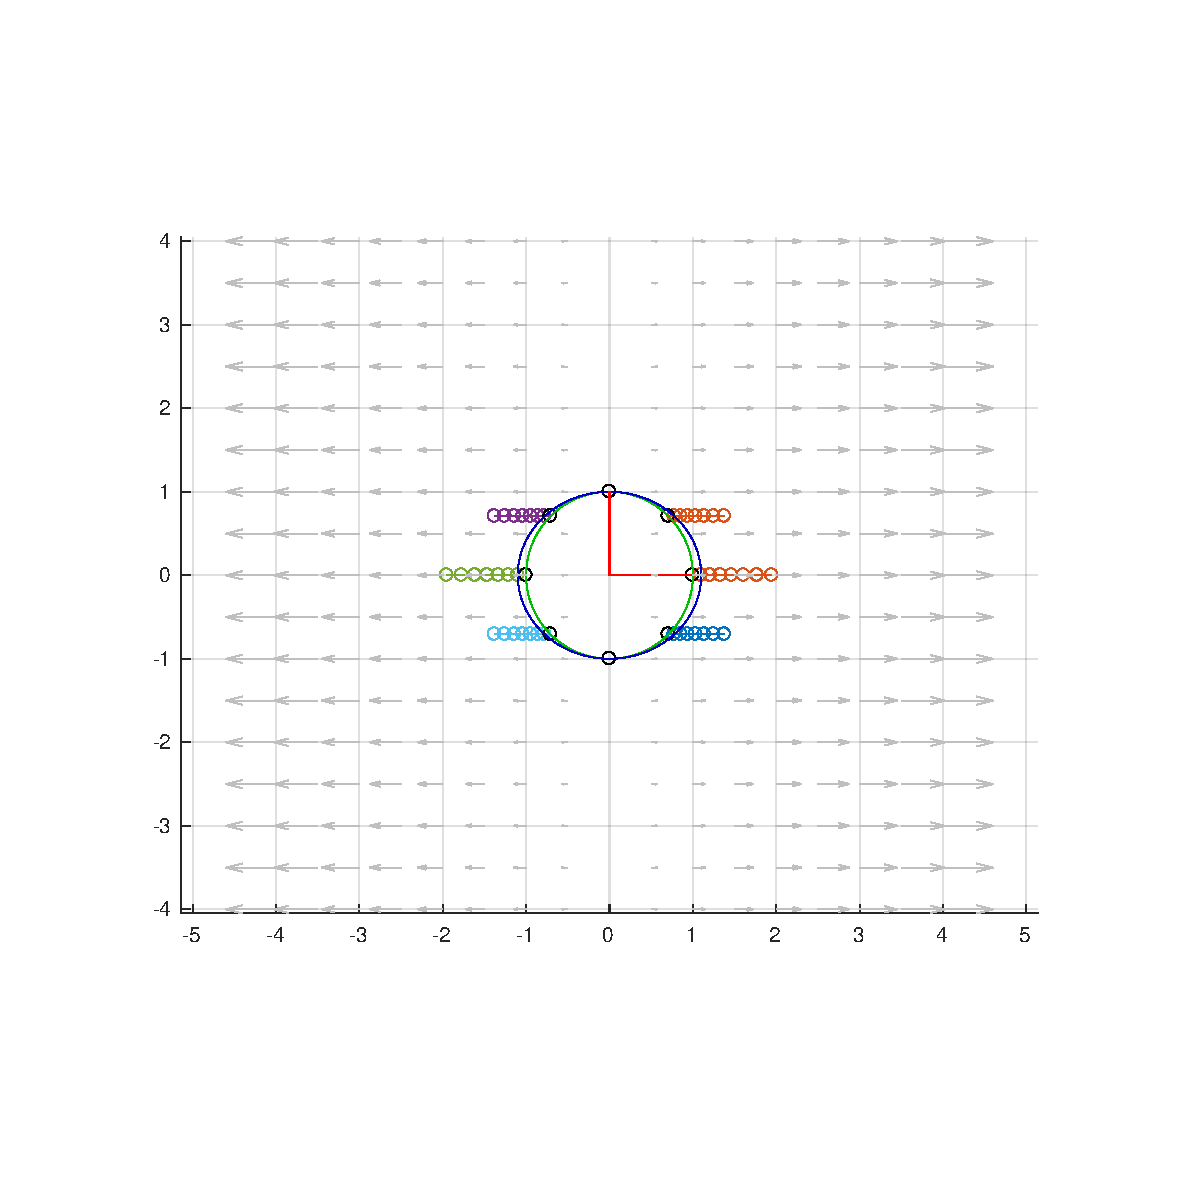
\includegraphics[width=0.99\linewidth]{const_11}
		\caption{$\lambda_1 = 1.1, \lambda_2 = 1 $}
		\label{fig:const3}
	\end{subfigure}%
	\caption{Badanie stabilności przez zmiane tylko jednej wartości widma}
	\label{figcons2}
\end{figure}

Jeśli wartości własne $ \lambda_1 = \lambda_2 = 1 $ to układ jest stały i przekształca samego w siebie. Jeśli zmniejszymy choć trochę wartość własną to w tym miejscu układ zaczyna zbiegać do zera. Jeśli zwiększymy choć trochę tę wartość własną układ zaczyna się rozbiegać w tym miejscu. To pokazuje kryterium stabilności, przez ocenę promienia spektralnego \[ \rho(A) = \{max (|\lambda_i|) : \varphi_A(\lambda)\} \]

Układ jest:
\begin{itemize}
	\item niestabilny gdy $\rho > 1 $
	\item stabilny gdy $\rho = 1 $
	\item stabilny asymptotycznie gdy $\rho < 1 $
\end{itemize}

\begin{figure}[H]
	
	\centering
	\begin{subfigure}{.5\textwidth}
		\centering
		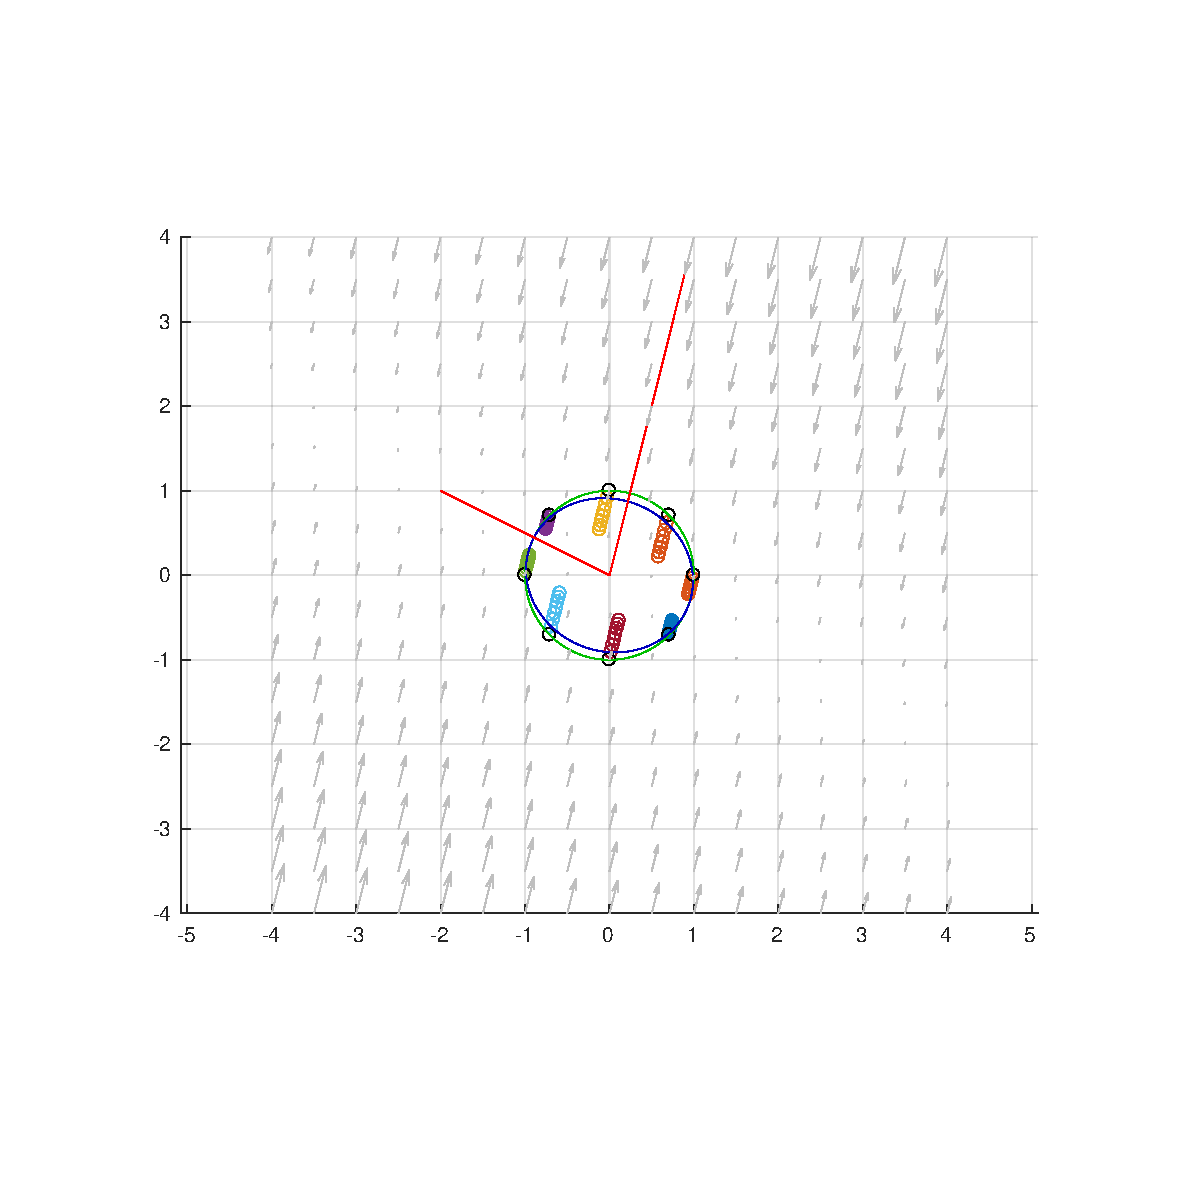
\includegraphics[width=0.99\linewidth]{const2_9}
		\caption{$\lambda_1 = 0.9, \lambda_2 = 1 $}
		\label{fig:const21}
	\end{subfigure}
	\begin{subfigure}{.5\textwidth}
		\centering
		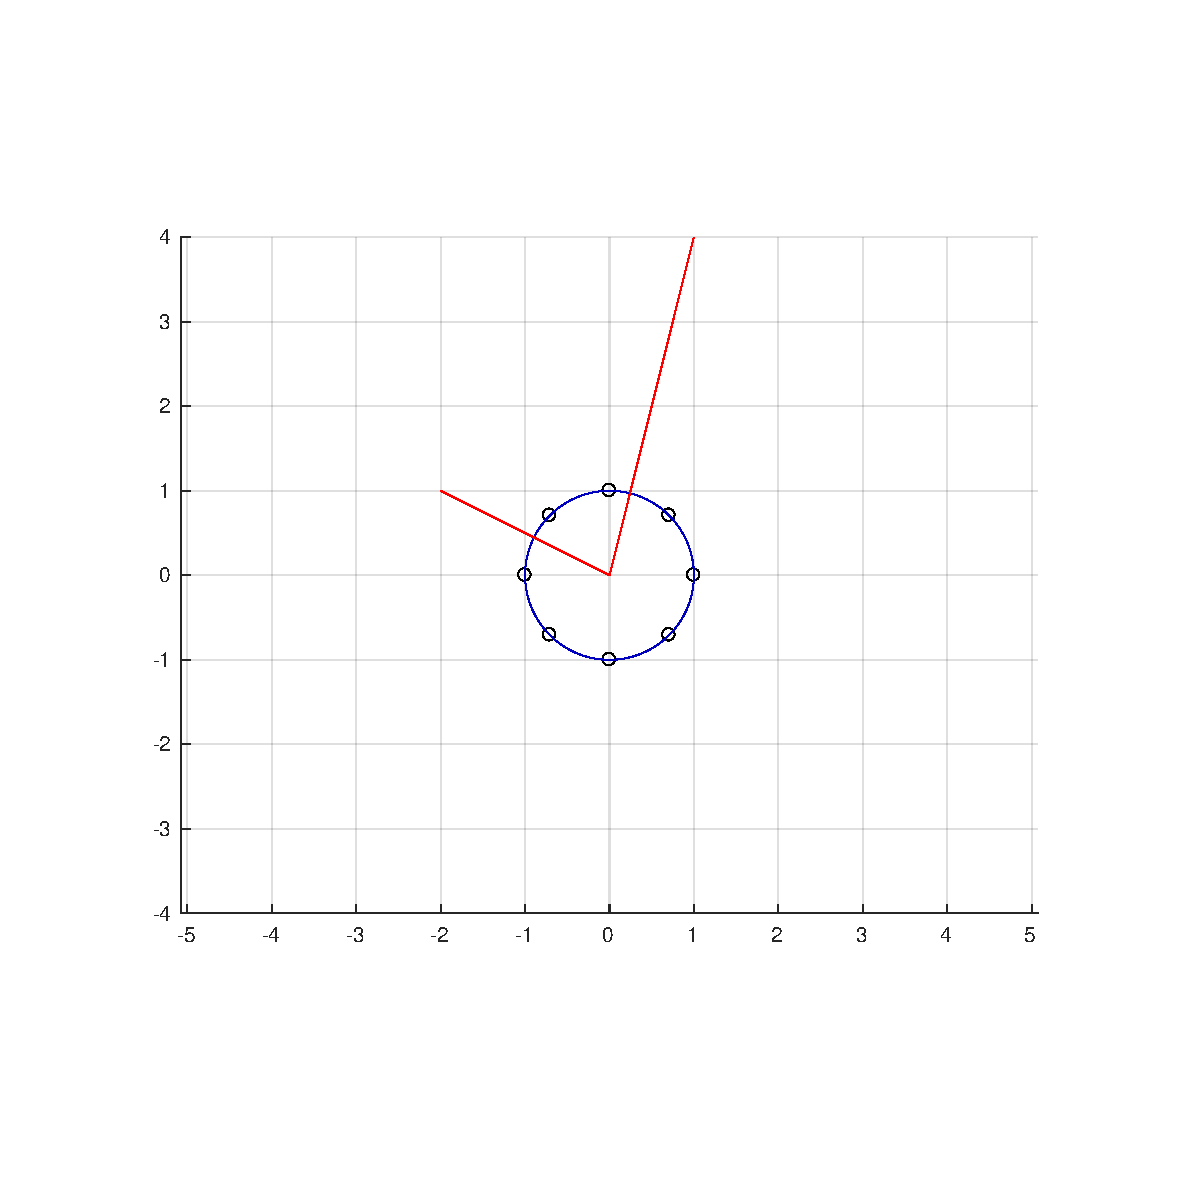
\includegraphics[width=0.99\linewidth]{const2_1}
		\caption{$\lambda_1 = 1, \lambda_2 = 1 $}
		\label{fig:const22}
	\end{subfigure}%
	\begin{subfigure}{.5\textwidth}
		\centering
		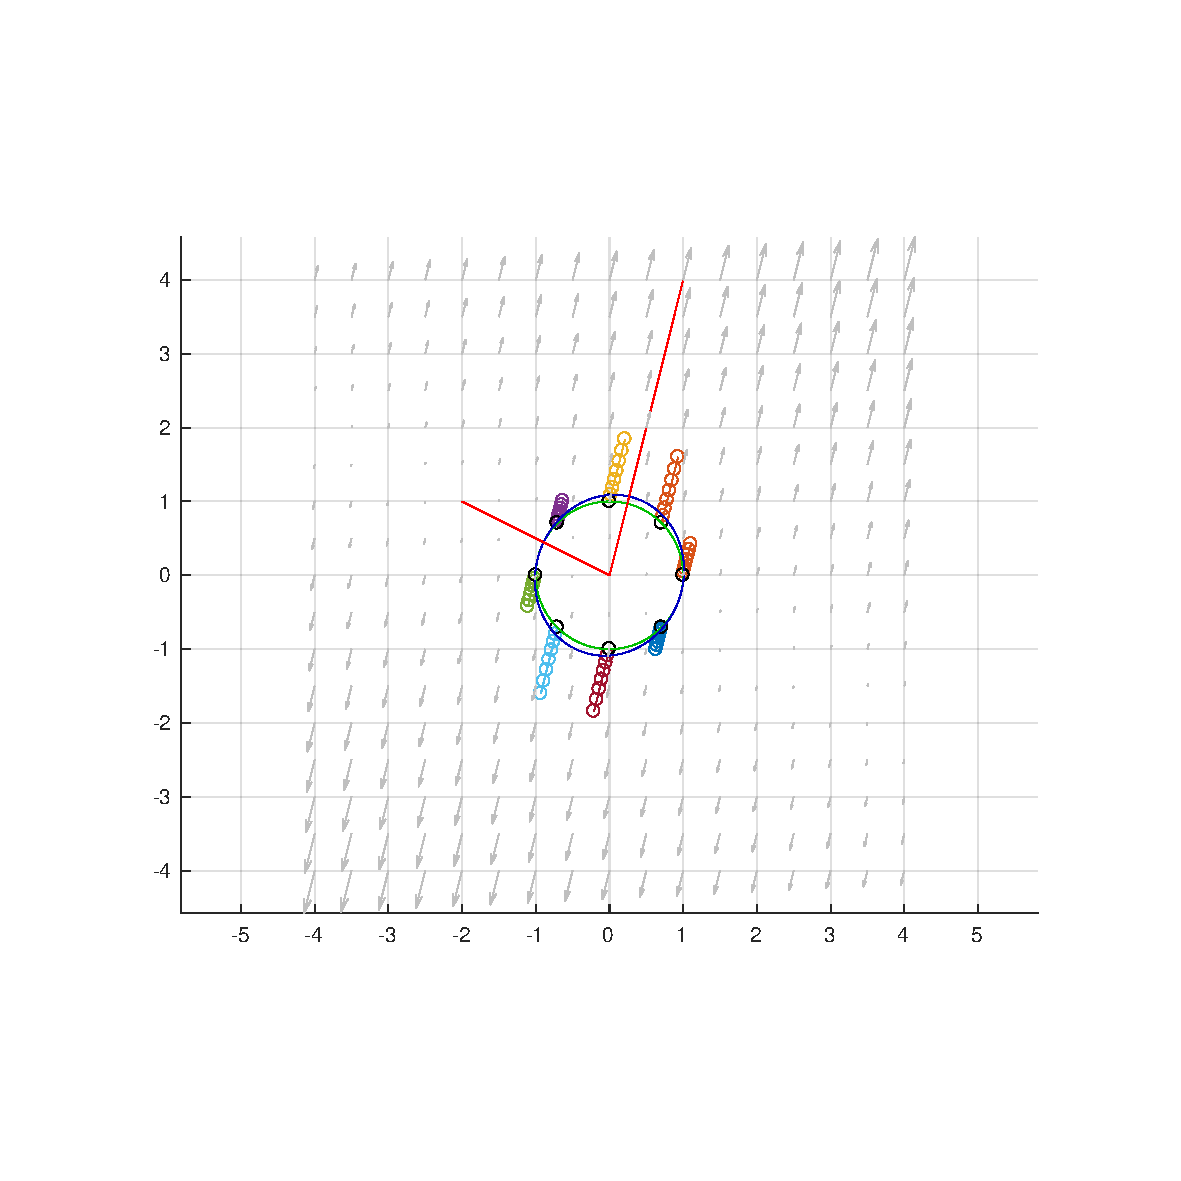
\includegraphics[width=0.99\linewidth]{const2_11}
		\caption{$\lambda_1 = 1.1, \lambda_2 = 1 $}
		\label{fig:const23}
	\end{subfigure}%
	\caption{Zmiana wektorów własnych nie zmienia stabilności, ale zmienia obrót}
	\label{figconst}
\end{figure}


\end{document}
